\chapter{Demonstration: Global Illumination}

\section{Results obtained}
\label{ResultsObtained}

\par
The developed application was tested in 5 different devices:

\begin{itemize}
	\item Samsung Galaxy Fresh Duos GT-S7392
	\item Raspberry Pi 2 Model B
	\item MINIX NEO X8-H PLUS (k200)
	\item Android Virtual Device (AVD) in a desktop
	\item Android Virtual Device in a laptop
\end{itemize}

\begin{table}[H]
	\small
	\centering
	\caption{Devices specifications}
	\label{specs}
	\hspace*{-3.3cm}
	\begin{tabular}{|l|l|l|l|l|}
		\hline
		Device&CPU&Cache(L1/L2/L3)&GPU&RAM\\ \hline
		Samsung Galaxy&1xARM Cortex A9 @1GHz&64KB/Unknown&1xBroadcom VideoCore IV&512MB\\ \hline
		Raspberry Pi 2 Model B&4xARM Cortex A7 @900MHz&64KB/1MB&1xBroadcom VideoCore IV&1GB\\ \hline
		MINIX NEO X8 PLUS&4xARM Cortex A9 @2.0GHz&64KB/Unknown&4xMali-450 MP&2GB\\ \hline
		AVD (desktop)&4xIntel Xeon CPU E5-1620 v4 @3.50GHz&64KB/256KB/10MB&1xNvidia Quadro P2000&16GB\\ \hline
		AVD (laptop)&4xIntel® Core™ i7-4710MQ @2.5GHz&64KB/256KB/6MB&1xNvidia 860M&16GB \\ \hline
	\end{tabular}
\end{table}

\par
As you can see in the table \ref{specs}, the application has been tested on a variety of devices.
Unfortunately, it was only possible to test it on 1 mobile device, the Samsung Galaxy Fresh Duos GT-S7392.
This device is a low-end smartphone with a low-end CPU with only 1 cpu core.

\par
It was also possible to test it on 2 different computers that are portable and even smaller than a common laptop.
The Raspberry Pi 2 Model B and the MINIX NEO X8-H PLUS which are devices with the Android operating system installed.

\par
Last, but not least, it was also tested in 2 Android Virtual Devices, 1 desktop and 1 laptop.
The desktop is a HP Z440 computer, which is a workstation, and the laptop is a Clevo W230SS, which is a middle end computer.

\begin{figure}[H]
	\centering
	\caption{Illustration of conference scene, rendered with shader Whitted in MobileRT.}
	\label{scene_conference}
	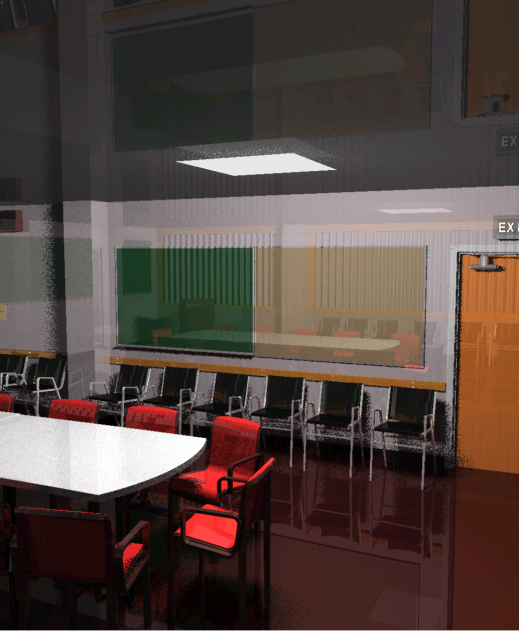
\includegraphics[keepaspectratio,scale=0.5]{Scene_Conference.png}
\end{figure}

\par
The scene used for testing was the conference scene, as illustrated in figure \ref{scene_conference}.
This scene consists of 331179 triangles and has 2 area lights in form of triangles.

\subsection{Raspberry Pi 2 Model B}

\begin{tikzpicture}
\begin{axis}[
legend style={at={(1.05,1.00)},anchor=north west},
axis lines = left,
xlabel = \#threads,
ylabel = speedup,
xtick={0,1,2,3,4},
ytick={0,1,...,10},
]
\addplot [
color=blue,
mark=*,
dashed,
] plot coordinates {
	(0,0.0)
	(1,1.0)
	(2,1.0)
	(3,1.0)
	(4,1.0)
};
\addlegendentry{Without Accelerator Structure}
\addplot [
color=black,
mark=*,
dashed,
] plot coordinates {
	(0,0.0)
	(1,1.0)
	(2,1.0)
	(3,1.0)
	(4,1.0)
};
\addlegendentry{Regular Grid}
\addplot [
color=red,
mark=*,
dashed,
] plot coordinates {
	(0,0.0)
	(1,1.0)
	(2,1.0)
	(3,1.0)
	(4,1.0)
};
\addlegendentry{Octree}
\label{graph:NoShadows}
\end{axis}
\end{tikzpicture}


\subsection{MINIX NEO X8-H PLUS}

\begin{tikzpicture}
\begin{axis}[
legend style={at={(1.05,1.00)},anchor=north west},
axis lines = left,
xlabel = \#threads,
ylabel = speedup,
xtick={0,1,2,3,4},
ytick={0,1,...,10},
]
\addplot [
color=blue,
mark=*,
dashed,
] plot coordinates {
	(0,0.0)
	(1,1.0)
	(2,1.0)
	(3,1.0)
	(4,1.0)
};
\addlegendentry{Without Accelerator Structure}
\addplot [
color=black,
mark=*,
dashed,
] plot coordinates {
	(0,0.0)
	(1,1.0)
	(2,1.0)
	(3,1.0)
	(4,1.0)
};
\addlegendentry{Regular Grid}
\addplot [
color=red,
mark=*,
dashed,
] plot coordinates {
	(0,0.0)
	(1,1.0)
	(2,1.0)
	(3,1.0)
	(4,1.0)
};
\addlegendentry{Octree}
\label{graph:NoShadows}
\end{axis}
\end{tikzpicture}

\subsection{Android Virtual Device in an ASUS desktop}

\begin{tikzpicture}
\begin{axis}[
legend style={at={(1.05,1.00)},anchor=north west},
axis lines = left,
xlabel = \#threads,
ylabel = speedup,
xtick={0,1,2,3,4},
ytick={0,1,...,10},
]
\addplot [
color=blue,
mark=*,
dashed,
] plot coordinates {
	(0,0.0)
	(1,1.0)
	(2,1.0)
	(3,1.0)
	(4,1.0)
};
\addlegendentry{Without Accelerator Structure}
\addplot [
color=black,
mark=*,
dashed,
] plot coordinates {
	(0,0.0)
	(1,1.0)
	(2,1.0)
	(3,1.0)
	(4,1.0)
};
\addlegendentry{Regular Grid}
\addplot [
color=red,
mark=*,
dashed,
] plot coordinates {
	(0,0.0)
	(1,1.0)
	(2,1.0)
	(3,1.0)
	(4,1.0)
};
\addlegendentry{Octree}
\label{graph:NoShadows}
\end{axis}
\end{tikzpicture}

\subsection{Android Virtual Device in a Clevo W230SS laptop}

\begin{tikzpicture}
\begin{axis}[
legend style={at={(1.05,1.00)},anchor=north west},
axis lines = left,
xlabel = \#threads,
ylabel = speedup,
xtick={0,1,2,3,4},
ytick={0,1,...,10},
]
\addplot [
color=blue,
mark=*,
dashed,
] plot coordinates {
	(0,0.0)
	(1,1.0)
	(2,1.0)
	(3,1.0)
	(4,1.0)
};
\addlegendentry{Without Accelerator Structure}
\addplot [
color=black,
mark=*,
dashed,
] plot coordinates {
	(0,0.0)
	(1,1.0)
	(2,1.0)
	(3,1.0)
	(4,1.0)
};
\addlegendentry{Regular Grid}
\addplot [
color=red,
mark=*,
dashed,
] plot coordinates {
	(0,0.0)
	(1,1.0)
	(2,1.0)
	(3,1.0)
	(4,1.0)
};
\addlegendentry{Octree}
\label{graph:NoShadows}
\end{axis}
\end{tikzpicture}

\section{Comparison with Android CPU Raytracer (\cite{Android_CPU_Raytracer})}

\par
Comparison ...